\chapter{Hardware}
    The hardware side consists of two mechanically connected but kinematically independent goniometer stages, static mounting components and an electrical part.
    The electronics are subdivided into the power supply, motion and logic handling and an interface between XRS/detector/motion system and the logic.

    \section{Mechanics}
        Mechanically the main challenge is to build two co-axial and co-planar but kinematically independent operating goniometer stages.
        One to move the detector and one to move the specimen about there mutual center of rotation as shown in~\cref{fig:rough sketch of the motion system}.
        \begin{figure}[h]
            \centering
            \includesvg[width=.6\textwidth]{drawings/sketch_stages}%
            \caption[Rough sketch of the motion system.]{Rough sketch of the motion system.}%
            \label{fig:rough sketch of the motion system}%
        \end{figure}
        The light bulb depicted in~\cref{fig:rough sketch of the motion system} represents the XRS, the eye represents the detector and the specimen to analyze is positioned in the center\footnote{Clearly, an X-Ray source most likely will not be found in the fashion of an actual incandescent light bulb. Here, it merely serves as a visual shortcut representing a photon source. Furthermore, an actual eye performs rather poor at detecting \(\gamma\)-radiation. Thus, it, as well, shall serve the purpose of representation.}.
        The center stage varies the angle~\(\theta\) which is the angle spun between the incident beam path and the plane of the specimen.
        The detector stage~--~the outer circle in~\cref{fig:rough sketch of the motion system}~--~gets positioned along an angle~\(\varphi\).\par\medskip

        While both stages need to be capable of accurate and repeatable positioning, the detector stage needs to accelerate and carry the mass of the actual detector and its supporting structure.

        The rise of desktop 3D-printing and the growing communities around highly sophisticated open source/hardware machines made components for high precision yet low cost motion systems in the low to lower-mid power range more available than ever.
        Hence, common 3D-printer parts where used where applicable.
        To achieve accuracy a gearing system utilizing stepper motors, purpose made timing pulleys and timing belts with a GT3 profile and~\qty{2}{\milli\metre} pitch are chosen~\cite{Manual.POWERGRIPGT3,Manual.LIGHTPOWERPRECISION}.
        
        Besides other factors, to maintain repeatability the easiest ones to achieve are reduced springiness in the whole motion system by choosing good quality, glass-fiber lined timing belts and eliminating slip during changes of torque e.g. direction changes and/or acceleration and deceleration by means of preloading the drive system.\par\medskip

        A detailed description of the in this work proposed solutions are discussed in~\cref{sec:sample stage,,sec:detector stage}.
        
        \subsection{Sample Stage}\label{sec:sample stage}
            \Cref{fig:xmagix full sample highlightes} shows the main kinematic assembly and the sample stage with drive highlighted in light blue.
            \begin{figure}[ht]
                \centering
                \includesvg[width=.6\textwidth]{drawings/X-MAGIX_full_sample}%
                \caption[Full motion system. Sample stage blue highlighted.]{Full motion system. Sample stage highlighted in light blue.}%
                \label{fig:xmagix full sample highlightes}%
            \end{figure}%

            The center part of the main assembly is the slewing ring \textit{PRT-01-60} by \textsc{igus}~\cite{Manual.IglidePRTPolymerSlewingRings.} depicted as no. 6 in the section view in~\cref{fig:sample stage exploded section}.
            Its relatively large center hole gives room to place a smaller bearing assembly co-axially to its own axis of rotation.\par\medskip

            The stationary part of slewing ring provides two circular patterns of tapped bores fitting 10 M5 fasteners each.
            The holes along the inner circle are free to use.
            \textit{Stator center} (no. 7) is inserted into the slewing ring and hold in place by seven M5x10 bolts (no. 13).
            Hereafter and in that sequence, the \textit{stator center spacer} (no. 5) and ball bearing \textit{W 61708-2RS1} get inserted into the free space from the top.
            One secures the ball bearing press-fitting six of the \textit{stator locks} into there respective slots\footnote{ "Abusing" an ordinary drill-press to~--~well~--~press them in place (turned off!) works perfect.}.
            \begin{figure}[h]
                \centering
                \includesvg[width=.5\textwidth]{pictures/footage/stage_bearings}
                \caption[Detailed photo of the stator center]{Detailed photo of the stator center. Zoomed in a detailed view of the press-in-place stator center locks (1). At the top and bottom are the \textit{W 61708} bearings visible (2) with the \textit{stator center spacer} in between. The outer part is the \textit{stator center} itself. All parts except the bearings are 3D-printed in ABS.}
                \label{fig:detailed view of the stator center}
            \end{figure}
            With slight force the remaining bearing gets fit in place from the bottom against the \textit{stator center spacer} as well.
            
            Finally, the \textit{sample driven gear} (no. 14) and the \textit{endstop bump sample} (no. 11) together are tightened against the \textit{sample platform} (no. 2) which is placed into the bearings beforehand.
            In order to guide the timing belt later, two bearings stacks are screwed from the bottom into two adjacent tapped holes.

            \begin{figure}[h]
                \centering
                \includesvg[width=.8\textwidth]{drawings/sample_stage_-_exploded_section}%
                \caption[Sample stage exploded view~-~sectioned.]{Sample stage exploded view~-~sectioned. 1: Sample Platform, 2: Sample Driven Gear 80T, 3: W 61708, 4: Stator Center, 5: Stator Center Spacer, 9: M5 Hex nut, 10: M5x25, 13: Washer 5.3, 16: 635-2RS, 17: Endstop Bump Sample, 19: M5x55, 20: M5x50, 21: Stator Center Spacer Lock, 22: M5x10, 24: PRT-01-60.}%
                \label{fig:sample stage exploded section}%
            \end{figure}%
            Not shown in~\cref{fig:sample stage exploded section} is the driving sub-assembly for the sample stage.
            Since its assembly is considered straight forward and a more complex version is shown in~\cref{fig:detector drive exploded} an assembled view is found in~\cref{fig:sample drive} for reference.

        \subsection{Detector Stage}\label{sec:detector stage}
            The components comprising the detector stage are depicted in~\cref{fig:xmagix full detector highlightes}.
            Its principle of operation follows the same basic concept~--~a timing belt mechanically couples the driving sub-assembly on the right-hand side to the movable central platform.
            \begin{figure}[ht]
                \centering
                \includesvg[width=.6\textwidth]{drawings/X-MAGIX_full_detector}%
                \caption[Full motion system. Detector stage blue highlighted.]{Full motion system. Detector stage blue highlighted.}%
                \label{fig:xmagix full detector highlightes}%
            \end{figure}

            Again, the detector stage is subdivided into a driving sub-assembly as shown in~\cref{fig:detector drive exploded} and driven one shown in~\cref{fig:detector stage exploded} respectively.
            The driven portion of the detector stage only consists of two main parts mounted to the slewing ring.
            The \textit{detector platform} (no. 4) which is placed on the top at an arbitrary orientation and the \textit{detector driven gear} on the bottom of the slewing ring.
            \textit{M5x25} bolts and \textit{hex nuts} are placed into all holes but the two where the \textit{endstop bump detector} (no. 6) is mounted.
            Here, to accommodate the needed extra length, \textit{M5x30} bolts are used instead.
            The \textit{endstop bump detector} itself is oriented such that its outermost mounting hole is aligned with the hole at the clockwise end of the detector arm.
            To lift the detector to a suitable height above the \textit{sample platform }, \textit{detector spacers} are placed underneath the \textit{detector}.\par\medskip
            \begin{figure}[t]
                \centering
                \includesvg[width=.8\textwidth]{drawings/detector_stage_-_exploded}%
                \caption[Detector stage exploded view.]{Detector stage exploded view. 9: M5 Hex Nut, 10: M5x25, 23: XRS-A, 25: Detector Platform, 26: Detector Driven Gear 250T, 29: Endstop Bump Detector, 30: Detector Spacer, 31: M3x25, 42: M5x30.}%
                \label{fig:detector stage exploded}%
            \end{figure}
            
            \Cref{fig:detector drive exploded} shows an exploded view of the detector drive sub-assembly.
            The core component, a NEMA17 \num{200} steps per revolution stepper motor (no. 7), is placed on the inside of the housing (no. 27) and held in place by four \textit{M3x6} screws.
            Slotted srew holes allow easier installation of the timing belt and adjustment of tension later on.
            Together with a \textit{hex nut} and the \textit{belt tensioner} (no. 8), a \textit{M5x25} bolt allows to hold the motor in place while tensioning the belt prior to finally tightening the screws at the top.
            Bearing stacks identical to those seen in \cref{fig:sample stage exploded} are put in place to confine the belt path along a \qty{180}{\degree} loop around the \textit{80T} timing pulley (no. 28).
            Having as many teeth of the belt engage the pulley at any given time is preferred as it ensures good torque transmission without belt slipping at a lower overall belt tension and thus lower load on the motors.
            \begin{figure}[h]
                \centering
                \includesvg[height=.5\textheight]{drawings/detector_drive_-_exploded}
                \caption[Detector stage drive~-~exploded view.]{Detector stage drive~-~exploded view. 7: 17HM19-2004S, 8: Belt Tightener, 9: M5 Hex nut, 10, M5x25, 11: Washer 3.2, 12: M3x6, 13: Washer 5.3, 14: Motor Mount Socket, 16: 635-2RS, 27: Motor Mount Detector Drive, 28: GT3 2mm 80T.}
                \label{fig:detector drive exploded}
            \end{figure}

        \subsection{Base and X-Ray Source}
            \lipsum

    \section{Electronics}
        On the electronics side, several tasks need to be accomplished.
        Most basic of which is powering each of the systems components.
        The SBC is typically powered via its dedicated USB-C port which in turn requires a \qty{5.1}{\volt} supply with a recommended current rating of \qty{3}{\ampere}~\cite{Manual.Documentation.RPF}.
        The detectors specifications state, that it needs a \qty{5}{\volt} power supply and draws less than \qty{3}{\watt} which translates to \(<\qty{0.6}{\ampere}\).
        Taken from the datasheet, the XRS is driven by an input voltage of \qty{24}{\volt} and an input current of \qty{1.1}{\ampere}~\cite{Manual.MAGPRODataSheet.QD}.
        The two stepper motors are each driven by TMC2209 stepper drivers which in turn accept a relatively broad range of \qtyrange{4.75}{29}{\volt}~\cite{Manual.TMC2209Datasheet} as supply voltages.
        The remaining peripherals such as the interface between the SBC and the XRS are directly driven from \qty{3.3}{\volt} and \qty{5}{\volt} provided by the Raspberry Pi's GPIO-Header.

        A tabulated summery of the supply power requirements can be found in \cref{tab:power requirements}.\par\medskip
        \begin{table}[h]
            \centering
            \caption[Electrical power requirements of the various installed components]{Electrical power requirements of the various installed components.}%
            \label{tab:power requirements}
            \begin{tabular}{@{}lSS@{}}
                \toprule
                Component&  {Voltage / \unit{\volt}}&    {Current / \unit{\ampere}}\\
                \midrule
                SBC&            5.1&    3.0\\
                Detector&       5.0&    0.6\\
                XRS&            24.0&   1.1\\
                Motor Driver&   24.0&   3.0\\
                \bottomrule
            \end{tabular}
        \end{table}

        Following the above considerations, a \qty{5}{\volt} \qty{25}{\watt} PSU (\textit{RS-25-5}) and a \qty{24}{\volt} \qty{150}{\watt} PSU (\textit{LRS-150-24}) are installed.
        Each is able to deliver slightly more power than expected to be necessary.
        Thus, leaving headroom for future extensibility and peaks in power demand.
        The single \qty{24}{\volt}-PSU supplying the stepper drivers and the XRS minimizes complexity and reduces costs.\par\medskip

        All wiring~--~where applicable~--~is routed through perforated cable ducting.

        \subsection{Kinematics}

        \subsection{Raspberry Pi to X-Ray Source Interface}
            The most straight forward way of operating and monitoring the XRS would be connecting to its dedicated USB-B port and using there GUI tool ``12WattController''.
            It allows to set and monitor the tubes acceleration voltage as well as the filament current, monitoring the devices on/off state, parametrizing and activating PWM operation mode and setting up an auto-shutdown timer.
            Unfortunately, the software only runs under \textsc{Microsoft} Windows and there are no means of accessing the control schemes programmatically.\par\medskip

            Located next to the USB-B port is a 2x5 Pin connector allowing analog control of the device and monitoring its state%
            \footnote{%
            MNF-No. \textit{IPL1-105-01-L-D-RA-K} according to the XRS manual.%
            }.
            \Cref{tab:xrs 10pin connector specs} is taken directly from the technical user guide included with the XRS:%
            \footnote{%
            Unfortunately, neither the manufacturer \textsc{Moxtek}, nor the reseller \textsc{Quantum Design Europe} provide freely accessible resources besides the cited data sheets~\cites{Manual.MAGPRODataSheet.MOXTEK}{Manual.MAGPRODataSheet.QD}.
            Therefore, this work will only provide contextual necessary transcripts of relevant parts of the included documents.%
            }
            \begin{table}
                \centering
                \caption[Pinout of the analog control connector of the XRS]{Pinout of the analog control connector of the XRS. Transcribed from the included users manual.}%
                \label{tab:xrs 10pin connector specs}
                \begin{tabular}{@{}llll@{}}
                    \toprule
                    Pin&    Functionn&      I/O Value&                                                          Response/Description\\
                    \midrule
                    1&      HV Enable&      \qtyrange{0.0}{+5.0}{\volt} (Input \(Z = \qty{10}{\kilo\ohm}\))&     \(< \qty{1.0}{\volt} = \text{OFF, } >\qty{4}{\volt} = \text{ON}\)\\
                    2&      Filament Ready& \qtyrange{0.0}{+5.0}{\volt} (Output \(Z = \qty{1}{\kilo\ohm}\))&     \(< \qty{1.0}{\volt} = \text{Not ready, } \qty{5}{\volt} = \text{Ready}\)\\
                    3&      HV Control&     \qtyrange{0.27}{+4.0}{\volt} (Input \(Z = \qty{100}{\kilo\ohm}\))&   \qtyrange{4}{60}{\kilo\volt}\\
                    4&      HV Monitor&      \qtyrange{0.27}{+4.0}{\volt} (Output \(Z = \qty{100}{\ohm}\))&       \qtyrange{4}{60}{\kilo\volt}\\
                    5&      Current Control& \qtyrange{0.04}{+4.0}{\volt} (Input \(Z = \qty{100}{\kilo\ohm}\))&   \qtyrange{10}{1000}{\micro\ampere}\\
                    6&      Current Monitor& \qtyrange{0.0}{+4.0}{\volt} (Output \(Z = \qty{100}{\ohm}\))&        \qtyrange{0}{1000}{\micro\ampere}\\
                    7&      Ground&         Ground&                                                             Ground\\
                    8&      Ground&         Ground&                                                             Ground\\
                    9&      Filament Enable&\qtyrange{0.0}{+5.0}{\volt} (Input \(Z = \qty{10}{\kilo\ohm}\))&     \(< \qty{1.0}{\volt} = \text{OFF, } >\qty{4}{\volt} = \text{ON}\)\\
                    10&     Input Power&    \(\qty{24}{\volt} \pm \qty{5}{\percent}\)&  Input Power\\
                    \bottomrule
                \end{tabular}
            \end{table}
            Pins 1, 3, 5 and 9 are inputs of which pins 1 and 9 are digital controls.
            ``Current Control'' and ``HV Control'' are set by manipulating the voltage levels on pins 3 and 5.
            The SBC only provides pseudo-analogous control via in-build hardware PWM \textquote{available on GPIO12, GPIO13, GPIO18, GPIO19}~\cite{Manual.Documentation.RPF}.
            PWM-control works by switching between logic-Hi and logic-Lo at a set frequency while varying the ratio between the times the signal is in Hi-state and Lo-state during one period.
            While this is acceptable with sufficiently slow reacting systems i.e. systems exhibiting low-pass behavior such as speed-control of brushed DC-Motors or brightness control of an LED taking advantage of the refresh rate of the human visual system, achieving a stable and reliable control of the XRS by means of PWM is highly unlikely.\par\medskip

            Due to time restrictions a rather crude interface board was made utilizing a two-channel digital-to-analog converter (DAC) for writing to and a two-channel analog-to-digital converter (ADC) for reading from the XRS.
            \begin{figure}[h]
                \centering
                \includesvg[width=.6\textwidth]{electronics/pdf/DAC_circuitry}
                \caption[Schematic of the DAC]{Schematic of the DAC.}
                \label{fig:DAC schematic}
            \end{figure}
            To generate analog signals a \textit{TLV5618A} was used.
            It integrates two separate output channels with 12bit resolution, delivers peak output voltages ranging from \qtyrange{2.7}{5.5}{\volt} and is SPI programmable~\cite{Manual.DAC.TLV5618A}.
            The schematic depicted in \cref{fig:DAC schematic} shows its external circuitry and the configuration of its voltage reference.
            In order to prevent clipping of the output voltage, it is important to keep the reference voltage below \(\frac{V_{DD} - \qty{0.4}{\volt}}{2}\) which effectively means keeping it below half the maximum desired output voltage~\cite[p. 3]{Manual.DAC.TLV5618A}.
            The used \textit{LT1009} delivers a sufficiently stable reference voltage of \(\approx \qty{2.385}{\volt}\) while pin 3 is tied to ground (see \cref{fig:LT1009 sim} for spice simulation analysis).
            Although this still is slightly higher than the limits stated above, minimal clipping of the output voltage should not be of a concern.
            Taken from \cref{tab:xrs 10pin connector specs} HV Control and Filament Control are ranging from \qtyrange{0.27}{4}{\volt} which limits the usable number of bits (\(UNOB\)) to:
            \begin{align}
                UNOB_{HV,Ctrl} &= UNOB_{HV,Ctrl,H} + UNOB_{HV,Ctrl,L} \nonumber\\
                &= \cint*{\frac{n_{bits}-1}{V_{DD}-\qty{0.4}{\volt}} \cdot \qty{0.6}{\volt}} - \cint*{\frac{n_{bits}-1}{V_{DD}-\qty{0.4}{\volt}} \cdot \qty{0.27}{\volt}} \nonumber\\
                &= 535 + 241 = 776
                \label{eq:UNOB hv DAC}
            \end{align}
            with \(UNOB_{HV,Ctrl,L}\) being the unusable number of bits between \qty{0}{\volt} and \qty{0.27}{\volt} and \(UNOB_{HV,Ctrl,H}\) the bits mapping the unusable range from \qtyrange{4}{4.6}{\volt}.
            Calculating \(UNOB\) for Current Control yields
            \begin{equation}
                UNOB_I = 535 + 36 = 571
                \label{eq:UNOB filament DAC}
            \end{equation}
            with a resulting HV Control resolution
            \begin{equation}
                V_{Ctrl}(bit) = \frac{V_{Ctrl,max} - V_{Ctrl,min}}{n_{bits}} \approx \qty{13.7}{\volt\per\bit}
                \label{eq:HV ctrl resolution}
            \end{equation}
            and a Current Control resolution
            \begin{equation}
                I_{Ctrl}(bit) = \frac{I_{Ctrl,max} - I_{Ctrl,min}}{n_{bits}} \approx \qty{0.24}{\micro\ampere\per\bit}
                \label{eq:Current ctrl resolution}
            \end{equation}
            respectively.\par\medskip

            The analogous feedback values are sampled by an \textit{MCP3202}.
            The \textit{MCP3202} is a \qty{12}{\bit} two-channel ADC with an input range of \qtyrange{2.7}{5.5}{\volt} and SPI-programmable as well~\cite{Manual.ADC.MCP3202}.
            It uses its power supply as its voltage reference, thus, the \textit{LT1009} needs to be replaced in favor of a \qty{5}{\volt} reference.
            As shown in \cref{fig:ADC schematic}, a reference of type \textit{LM4040DIZ-5.0} is used.
            To provide a reference of \(\qty{5}{\volt} \pm \qty{2}{\percent}\), a cathode current of \qtyrange{0}{25}{\milli\ampere} must not be exceeded~\cite{Manual.LM4040PrecisionMicropowerShuntVoltageReference}.
            \begin{equation}
                I_Z = \frac{U_S - U_Z}{I_Z + I_L}
                \label{eq:LM4040 cathode current}
            \end{equation}
            With an assumed supply voltage slightly higher than nominal \qty{5}{\volt}, a maximum expected load current of \qty{550}{\micro\ampere}\footnote{Operating current of the \textit{MCP3202}.} and values given in the datasheet a current limiting resistor of \(\approx \qty{6}{\ohm}\) is calculated and reflected in the two parallel resistors \(R_4\) and \(R_5\) of \qty{12}{\ohm} each.
            \begin{figure}[h]
                \centering
                \includesvg[width=.65\textwidth]{electronics/pdf/ADC_circuitry}
                \caption[Schematic of the ADC]{Schematic of the ADC.}%
                \label{fig:ADC schematic}
            \end{figure}\par\medskip
            %
            With \(V_{DD} = V_{Ref,ADC}\), full scale of~\(V_{DD} - 1\cdot LSB\) and following the same considerations as in~\crefrange{eq:UNOB hv DAC}{eq:Current ctrl resolution} the ADC's~\(UNOB\) computes as follows:
            \begin{align}
                UNOB_{HV,Mon} &= \cint*{ \frac{2^{12}-1}{\qty{5}{\volt}} \cdot \qty{1}{\volt}} + \cint*{\frac{2^{12}-1}{\qty{5}{\volt}} \cdot \qty{0.27}{\volt}}\nonumber\\
                &= 819 + 222 = 1041
                \label{eq:UNOB hv ADC}
            \end{align}
            and
            \begin{equation}
                UNOB_{I,Mon} = 819 + 33 = 852
                \label{eq:UNOB current ADC}
            \end{equation}
            accordingly.
            With the HV~Monitors range being identical to the HV~Control range, HV Monitor reads with an equal resolution as in~\cref{eq:HV ctrl resolution}.
            Current Monitor instead misses an offset.
            With \cref{eq:Current ctrl resolution} and~\(I_{Mon,min} = \qty{0}{\micro\ampere}\) the Current monitor readings resolve to about~\qty{24.4}{\micro\ampere\per\bit} (\cref{eq:Current monitor resolution}).
            \begin{equation}
                I_{Mon}(bit) = \frac{I_{C,Mon,max}}{n_{bits}} \approx \qty{24.4}{\micro\ampere\per\bit}
                \label{eq:Current monitor resolution}
            \end{equation}\par\medskip

            \Cref{fig:top view interface board} shows the top view of the real-world implementation of the above.
            The yellow area~(1) comprises the DAC portion of the circuit, the purple area~(2) the ADC.
            The 10pin headers on the left and right connect to the SBC and the XRS.
            A detailed description of there respective pin-assignment can be found in the full schematics in~\cref{fig:schematics of peripherals}.
            The 2-pin connector on the upper-right receives~\qty{24}{\volt} to supply the XRS via pin 10 on its connector.
            \begin{figure}[h]
                \centering
                \includesvg[width=.7\textwidth]{pictures/footage/interface_front}
                \caption[Top view of the SBC-XRS-interface board]{Top view of the SBC-XRS-interface board. DAC in yellow (1), ADC in purple (2).}%
                \label{fig:top view interface board}
            \end{figure}
            The Pin ordering scheme for the 10-pin connector on the rear of the XRS is shown in \cref{fig:10 pin numbering scheme}.
            \begin{figure}[h]
                \centering
                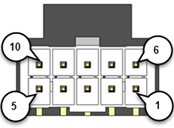
\includegraphics[width=.3\textwidth]{electronics/datasheets/XRS_10pin_male.png}
                \caption[XRS' analog control pin numbering scheme.]{XRS' analog control pin-numbering scheme.}%
                \label{fig:10 pin numbering scheme}
            \end{figure}